\documentclass[a4paper]{article}

\usepackage[czech]{babel} % základní podpora pro češtinu, mj. správné dělení slov
\usepackage[utf8]{inputenc} % vstupní kódování je UTF-8
\usepackage[T1]{fontenc} % výstupní kódování
\usepackage{fontspec} % řeší zahrnutí správných fontů pro LuaLaTeX a XeLaTeX
\usepackage[inline]{enumitem}
\usepackage{gensymb}
\usepackage{caption}
\usepackage{subcaption}
\usepackage{gensymb}
\usepackage{hyperref}
\usepackage[left=3cm,right=3cm,bottom=3.5cm]{geometry}
\usepackage{graphicx,lipsum}
\usepackage{amsmath}
\usepackage{array}
\usepackage{float}
\usepackage{cleveref}
\usepackage{siunitx}
\usepackage[table,xcdraw]{xcolor}
\usepackage{tabularx}
\usepackage{rotating}  % For sidewaysfigure and rotating content
\usepackage{adjustbox}
\usepackage{amsfonts} 
\usepackage{array}
\usepackage{fancyhdr} % For custom headers and footers
\usepackage{capt-of}   % For captions in minipage
\usepackage{graphicx}
\usepackage{listings}

\pagestyle{fancy}
\fancyhf{} % Clear default header and footer
% Header with section and subsection
\fancyhead[R]{\small\textcolor{gray}{\nouppercase{\leftmark}}} % Section name
%\fancyhead[R]{\small\textcolor{gray}{\nouppercase{\rightmark}}} % Subsection name

% Footer with a picture, author name, and some text
\fancyfoot[L]{\raisebox{-15pt}{
\includegraphics[width=2.5cm]{dokumentace/pic/FIT_trans.png}}}
\fancyfoot[C]{\thepage}
\fancyfoot[R]{\small\textcolor{gray}{Největší klika v neorientoaném grafu\\Lukáš Lev, 256660}} % Add your desired text
\renewcommand{\headrulewidth}{0pt}

% code snippets
\lstset{
  language=C,                     % Choose the language of the code
  basicstyle=\ttfamily\footnotesize, % Set font style and size
  keywordstyle=\color{blue},      % Style for keywords
  stringstyle=\color{red},        % Style for strings
  commentstyle=\color{gray},      % Style for comments
  numbers=left,                   % Add line numbers
  numberstyle=\tiny\color{gray},  % Style for line numbers
  stepnumber=1,                   % Line numbering step
  breaklines=true,                % Automatic line breaking
  frame=single,                   % Frame around the code
}

\begin{document}

\begin{titlepage}
    \begin{center}
        \vspace*{1cm}
            
        \Huge
        \textbf{Největší klika\\v neorientovaném grafu}
            
        \vspace{0.5cm}
        \LARGE
            
        \vspace{1.5cm}
            
        \textbf{Lukáš Lev}
            
        \vfill
            
        Semestrální práce\\
        IAL
            
        \vspace{0.8cm}
            
        
\includegraphics[width=0.4\textwidth]{dokumentace/pic/FIT.png}
            
        \Large
        UIFS\\
        VUT-FIT\\
        \today
        %28. 11. 2024
            
    \end{center}
\end{titlepage}
\newpage

\section{Zadání} \label{sec:zadani}
    Náhradní projekt je určen pouze pro studenty, kteří v předmětu IFJ neřeší souběžný projekt (např. studenti FEKT nebo studenti opakující předmět). Tento projekt je týmový a řeší jej trojice nebo čtveřice studentů.\\
    
    \noindent
    \textbf{Zadání varianty}\\
    \textit{Klika grafu} je podgraf, který je úplným grafem (=kterýkoliv vrchol kliky je tedy spojen hranou se všemi ostatními vrcholy kliky).\\
    \noindent
    Vytvořte program pro hledání největší kliky v neorientovaném grafu. Pokud existuje více řešení, nalezněte všechna. Výsledky prezentujte vhodným způsobem. Součástí projektu bude načítání grafů ze souboru a vhodné testovací grafy. V dokumentaci uveďte teoretickou složitost úlohy a porovnejte ji s experimentálními výsledky.\\
    
    \noindent
    \textbf{Všeobecné informace a pokyny k náhradním projektům}
    
    \noindent
    Řešení bude vypracováno v jazyce C a bude přeložitelné (pomocí příkazu make) na serveru eva.fit.vutbr.cz. Všechny zdrojové kódy, hlavičkové soubory, testovací data aj. budou logicky separovány a uloženy v příhodně pojmenovaných podadresářích. Použití nestandardních knihoven není dovoleno. Všechny části zadání varianty jsou nutnou součástí řešení.\\
    
    \noindent
    Celkové hodnocení projektu sestává z následujících kategorií:
    \begin{itemize}
        \item funkčnost implementace (až 6 bodů),
        \item projektová dokumentace (až 4 body),
        \item obhajoba (až 5 bodů).
    \end{itemize}
    
    \noindent
    Řešení zabalené v jediném ZIP archivu je odevzdáváno pouze vedoucím týmu prostřednictvím STUDISu. Závazné pokyny pro vypracování projektové dokumentace a doporučení pro závěrečné obhajoby naleznete v Moodlu v sekci Projekty.
    
\section{Abstrakt} \label{sec:abstrakt}
    Tento projekt byl proveden podle zadání z kapitoly \ref{sec:zadani}, jež bylo poskytnuto vyučujícím.\\
    
    \noindent
    Předmětem tohoto projektu je hledání \textbf{největší kliky v neorientovaném grafu}, což je jeden z typických problémů v teorii grafů \cite{max-cliq}. Tato problematika je krátce popsána v kapitole \ref{sec:zadani}.\\
    
    \noindent
    Pro hledání největší kliky v neorientovaném grafu byly navrženy dva algoritmy, a to sice
    \begin{itemize}
        \item algoritmus metodou hrubé síly (anglicky \textit{brute force}),
        \item algoritmus zpětného vyhledávání (anglicky \textit{backtracking}).
    \end{itemize}
    Pro každý z těchto algoritmů byla stanovena časová komplexita nejprve teoreticky a následně také experimentálně pomocí jednoduchého programu v jazyce C.
    
\section{Teorie} \label{sec:teorie}
    \subsection{Zkoumané objekty}
        \paragraph{Graf} je základní objekt teorie grafů. Skládá se z uzlů (vrcholů) a hran.\cite{slu_zaklad-teo-grafu}
        
        \paragraph{Neorientovaný graf}
        je graf, jehož všechny uzly jsou symetricky spojeny neorientovanou hranou.\cite{slu_zaklad-teo-grafu}
        
        \paragraph{Úplný graf} je neorientovaný graf, pro jehož každou dvojici vrcholů existuje právě jedna neorientovaná hrana.\cite{slu_zaklad-teo-grafu}
        
        \paragraph{Klika} (anglicky \textit{clique}) je podmnožina vrcholů neorientovaného grafu. Tato podmnožina tvoří úplný graf.\cite{cliq-definition}

    \subsection{Teorie použitých algoritmů} \label{subsec:complexities_teo}
        Tato kapitola se věnuje teoretickým vlastnostem použitých algoritmů metody hrubou silou a metody zpětného vyhledávání. Především pak jejich časovým a prostorovým složitostem. Implementace obou těchto algoritmů je kritická pro jejich složitost. Touto problematikou se zabývá kapitola \ref{sec:implem}.\\

        \noindent
        Kruciální pro tuto kapitolu je reprezentace grafu, kterou implementace používá. Jelikož graf je reprezentován pomocí matice sousednosti (kapitola \ref{subsec:graph_imp}) je velice těžké vyhnout se při řešení problému hledání největší kliky exponenciální složitosti.

        \subsubsection{Algoritmus metodou hrubé síly}
            \paragraph{Časová složitost:} Algoritmus iteruje každým možným podgrafem původního grafu o velikosti (počtu uzlů) $n$ a u každého z těchto podgrafů provádí zkoušku, zda jsou klikami, a to tak, že kontroluje každý uzel tohoto podgrafu. Oba tyto cykly mají vliv na časovou složitost algoritmu.\\[3pt]
            \noindent
            Protože pro konstrukci každého podgrafu musíme určit stav každého uzlu jako 1 (náleží podgrafu), nebo 0 (nenáleží podgrafu) - tedy vybrat ze dvou stavů, určíme počet všech možných podgrafů jako $2^n$. Dále stanovíme počet iterací vycházející z kódu (implementace je rozebrána v kapitole \ref{sec:implem}). Protože kód zabraňuje kontrole duplikátních dvojic uzlů v podgrafu, bude nejhorším možným počtem iterací kontrola pro podgraf o velikosti $n$. Z něj se vybere právě $\binom{n}{2} = \frac{n(n-1)}{2}$.\\[3pt]
            \noindent
            Časovou složitost tedy určíme zanedbáním konstant pro tyto vnořené cykly jako $\mathbf{O(2^n \cdot n^2)}$.

            \paragraph{Prostorová složitost:} podobně jako při určování časové složitosti vycházíme z toho, že pro každý možný podgraf ukládá implementace až $n$ možných klik (například pokud není mezi uzly žádná hrana). V nejhorším případě je tedy uloženo pro $2^n$ cyklů $n$ prvků. Prostorová složitost je tedy $\mathbf{O(2^n \cdot n)}$.

        \subsubsection{Algoritmus metodou zpětného vyhledávání}
            \paragraph{Časová složitost:} postup pro určení časové složitosti je obdobný jako pro algoritmus metodou hrubé síly. Největší možný počet vytvořených podgrafů je $2^n$, pokud by bylo pomocí zpětného vyhledávání natrefeno na výslednou kliku až jako poslední možný podgraf. Tentokrát však vnořený cyklus pro kontrolu zachování kliky iteruje nejhůře $n$-krát. Proto je časová složitost určena jako $\mathbf{O(2^n\cdot n)}$.

            \paragraph{Prostorová složitost:} pokud dojde k maximální rekurzi, vnoření proběhne právě $n$-krát. Pro ukládání právě analyzované kliky je zapotřebí pole o velikosti $n$. Obě tyto veličiny jsou však nezávislé na ukládání největších klik. V nejhorším případě je v grafu $2^n$ podgrafů o velikosti až $n$. Proto uvažujeme, že prostorová složitost je $\mathbf{O(2^n \cdot n)}.$ 

    \begin{minipage}{.5\textwidth}
        \centering
        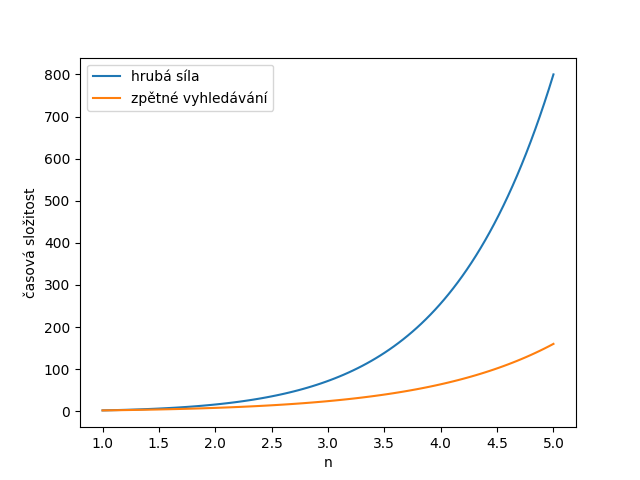
\includegraphics[width=1\linewidth]{dokumentace/exp_vyhodnoceni/theo_lin_lin.png}
        \captionof{figure}{Grafické vyjádření horní hranice časových složitostí obou algoritmů.}
        \label{fig:complx_theo_linlin}
    \end{minipage}
    \begin{minipage}{.5\textwidth}
        \centering
        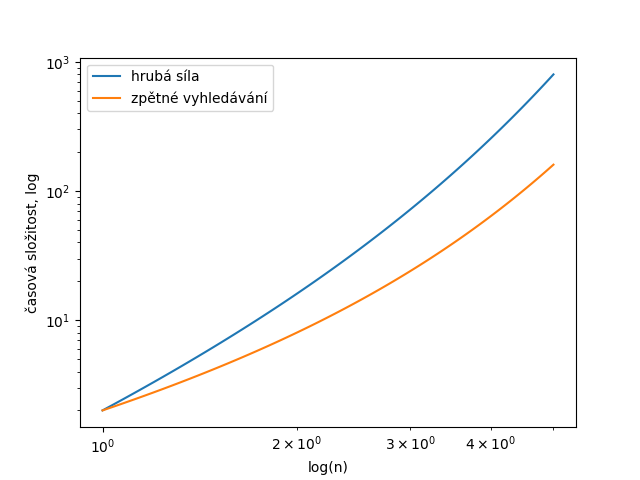
\includegraphics[width=1\linewidth]{dokumentace/exp_vyhodnoceni/theo_log_log.png}
        \captionof{figure}{Grafické vyjádření horní hranice časových složitostí obou algoritmů s logaritmickým škálováním na osách.}
        \label{fig:complx_theo_loglog}
    \end{minipage}
    

\section{Implementace v jazyce C}  \label{sec:implem}
    Podle zadání (kapitola \ref{sec:zadani}), byly oba algoritmy vypracovány v jazyce C. Další rysy implementace, které vycházejí ze zadání, se týkají zavedených datových struktur (kapitola \ref{subsec:graph_imp}). Implementace obou algoritmů vykazují požadované chování a v případě výskytu několika klik o maximální velikosti nacházejí všechny tyto výsledky. Zároveň, nenachází-li se v grafu žádná hrana, jsou nalezeny všechny vrcholy jako největší kliky.\\

    \subsection{Reprezentace neorientovaného grafu} \label{subsec:graph_imp}
        Podle zadání (kapitola \ref{sec:zadani}) je třeba vytvořit takovou datovou strukturu neorientovaného grafu, kterou lze snadno reprezentovat záznamem do jednoduchého souboru.\\

        \noindent
        Jednou z možných variant je \textbf{matice sousednosti}. Tato matice je čtvercová a, jelikož v rámci implementace neuvažujeme hrany uzlů vedoucí na sebe sama, hlavní diagonála této matice je nulová a matice je podle této diagonály symetrická. Pro ostatní prvky platí, že vyjadřují přítomnost hrany mezi uzly s indexem shodným s řádkem či sloupcem matice.\\

        \noindent
        Následující rovnice uvádí názorný příklad matice sousednosti (grafická reprezentace této matice je na obr. \ref{fig:graf1}). Prvky této matice jsou hrany mezi vrcholy označenými indexem. Tedy například prvek $h_{04} = 1$ tvrdí, že mezi uzly 0 a 1 se nachází hrana, zatímco mezi uzly 0 a 1 nikoliv ($h_{01} = 0$).

        \begin{equation} \label{eq:adj-mat}
            \mathrm{M_s} = 
            \begin{pmatrix}
                h_{00} & h_{01} & h_{02} & h_{03} & h_{04} \\
                h_{10} & h_{11} & h_{12} & h_{13} & h_{14} \\
                h_{20} & h_{21} & h_{22} & h_{23} & h_{24} \\
                h_{30} & h_{31} & h_{32} & h_{33} & h_{34} \\
                h_{40} & h_{41} & h_{42} & h_{43} & h_{44}
            \end{pmatrix} = 
            \begin{pmatrix}
                0 & 0 & 0 & 1 & 1 \\
                0 & 0 & 1 & 0 & 1 \\
                0 & 1 & 0 & 1 & 0 \\
                1 & 0 & 1 & 0 & 1 \\
                1 & 1 & 0 & 1 & 0
            \end{pmatrix}
        \end{equation}

        \noindent
        Zdrojový kód pro implementaci této matice se nachází v souboru \lstinline{graph.c}. V něm je definována struktura \lstinline{graph} popsaná níže.

        \begin{lstlisting}[caption={Definice struktury neorientovaného grafu.},captionpos=b]
typedef struct {
    int size;  // velikost matice (odpovida poctu uzlu)
    int** matrix;  // 2D pole pro ulozeni prvku matice
} graph;
        \end{lstlisting}

        \noindent
        Soubor \lstinline{graf.c} také obsahuje řadu funkcí vztahujících se k těmto grafům. Těmito funkcemi jsou:
        \begin{itemize}
            \item \lstinline{graph* graph_init(int size)} pro inicializaci prázdného grafu s vhodnou velikostí,
            \item \lstinline{void graph_delete(graph* g)} pro smazání grafu a uvolnění jeho paměti,
            \item \lstinline{int graph_read_size(const char* filename)} pro přečtení velikosti grafu (počtu uzlů) v matici sousednosti ze souboru,
            \item \lstinline{int graph_read(graph* g, const char* filename)} pro přečtení matice sousednosti ze souboru, vlastnosti grafu jsou uloženy do vstupní proměnné \lstinline{g} (nevyužívá funkci \lstinline{graph_read_size}),
            \item \lstinline{int graph_write(graph* g, const char* filename)} pro zápis matice sousednosti do souboru,
            \item \lstinline{void graph_print(graph* g)} pro vytištění grafu do terminálu
        \end{itemize}

        \noindent
        Soubory, které slouží pro ukládání grafu, jsou označeny příponou \lstinline{.gh} a matici sousednosti uchovávají v následujícím formátu, kde první řádek reprezentuje velikost matice a ostatní řádky informace o jejich prvcích:
        \begin{lstlisting}[caption={Zápis matice v \lstinline{.gh} souboru.},captionpos=b,label={code:zapis_matice}]
5
0 0 0 1 1
0 0 1 0 1
0 1 0 1 0
1 0 1 0 1
1 1 0 1 0
        \end{lstlisting}
        Tato matice je reprezentována také graficky na obrázku \ref{fig:graf1}.
        \begin{figure}[bh]
            \centering
            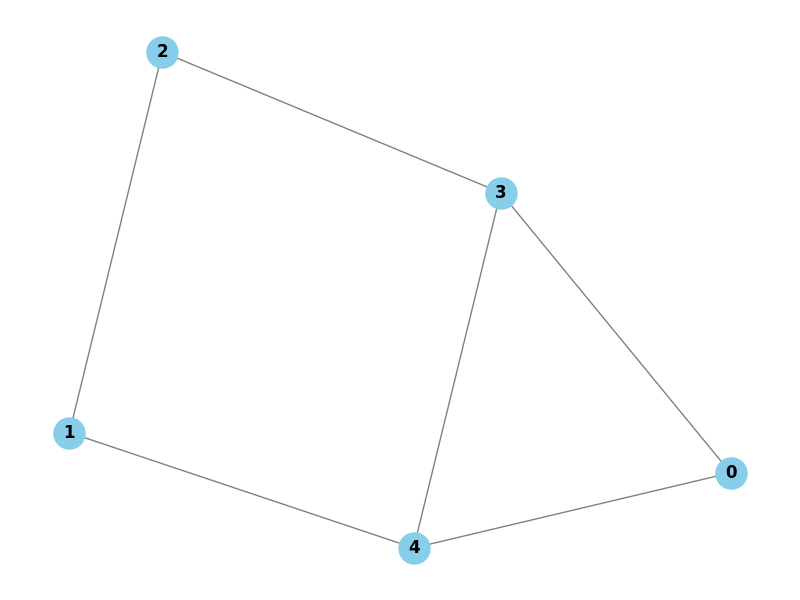
\includegraphics[width=0.5\linewidth]{dokumentace/pic/graf_1.png}
            \caption{Grafická reprezentace neorientovaného grafu z kapitoly \ref{subsec:graph_imp}.}
            \label{fig:graf1}
        \end{figure}

        \noindent
        Bližší popis implementovaného kódu je součástí komentářů v souboru \lstinline{graph.c}.

    \subsection{Implementace algoritmu metody hrubou silou}
        Zdrojový kód pro algoritmus hledání největší kliky v neorientovaném grafu metodou hrubé síly (anglicky \textit{brute force}) je obsahem souboru \lstinline{algorithms/bruteforce.c}. Kód operuje se strukturou definovanou v kapitole \ref{subsec:graph_imp}. Samotný soubor obsahuje podrobné komentáře, a tak je shrnutí implementace v této kapitole pouze zběžné.\\

        \noindent
        Protože matice sousednosti obsahuje pouze prvky s hodnotou 1 nebo 0, byla zvolena reprezentace vybrané podmnožiny vrcholů pomocí binární masky. Na tu je referováno celým číslem \lstinline{int subset}, které po převodu do binární soustavy určuje, které uzly jsou vybrány. Indexace se shoduje s indexací uzlů v matici.\\

        \noindent
        Například pro matici definovanou v souboru v ukázce kódu \ref{code:zapis_matice} použijeme masku \lstinline{subset} určenou číslem 10. Pro masku \lstinline{subset} tak platí:
        \begin{equation}
            10_{(10)} = 01010_{(2)} \implies u_{0}u_{1}u_{2}u_{3}u_{4}
        \end{equation}
        \noindent
        Proto jsou maskou vybrány vrcholy na indexech 1 a 3 graficky reprezentovány na obrázku \ref{fig:graf_maska}. Pro vytvoření všech podgrafů vstupního grafu definovaného maticí sousednosti stačí iterativně inkrementovat hodnotu masky od nuly až do hodnoty $\mathbf{2^{n}}$, kde $n$ je počet uzlů v grafu. Při iteraci těmito podgrafy stačí sledovat, zda jsou klikami, a pokud ano, pak také jejich velikost. Největší kliky jsou uchovávány v proměnné \lstinline{int** largest_cliques} ve funkci \lstinline{void bruteforce(graph* g)}.\\
        
        \begin{figure}[th]
            \centering
            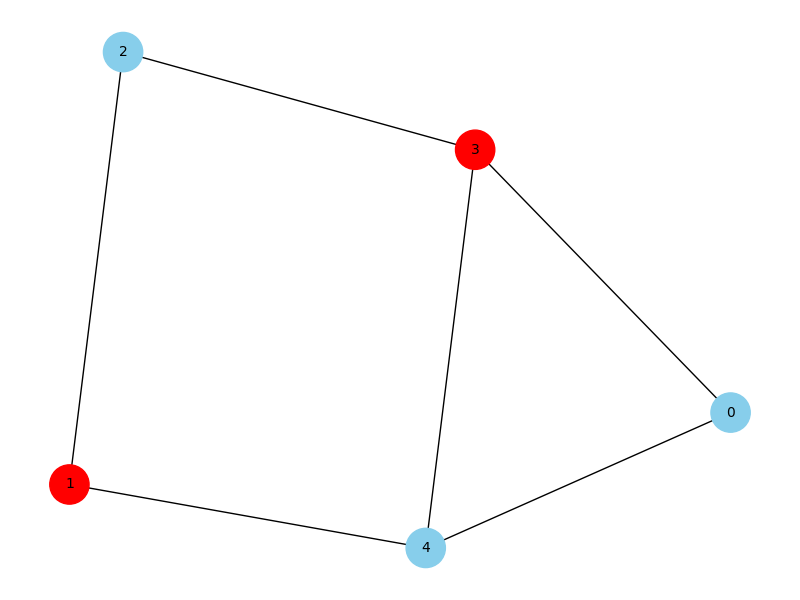
\includegraphics[width=0.5\linewidth]{dokumentace/pic/graf_1_13.png}
            \caption{Označení uzlů neorientovaného grafu maskou o hodnotě 10.}
            \label{fig:graf_maska}
        \end{figure}

        \noindent
        Soubor \lstinline{algorithms/bruteforce.c} obsahuje následující funkce:
        \begin{itemize}
            \item \lstinline{int is_clique_bruteforce(graph* g, int subset)} pro kontrolu, zda podgraf označený maskou \lstinline{subset} je klikou (zda je matice, krom diagonály, naplněna hodnotami 1),
            \item \lstinline{void bruteforce(graph* g)} pro iterativní hledání největší kliky. Tato funkce vytiskne všechny největší nalezené kliky do terminálu.
        \end{itemize}

    \subsection{Implementace algoritmu metody zpětného vyhledávání}
        Zdrojový kód pro hledání největší kliky v neorientovaném grafu pomocí metody zpětného vyhledávání je obsažen v souboru \lstinline{algorithms/backtracking.c}. V něm je pro tuto metodu použito následujících funkcí:
        \begin{itemize}
            \item \lstinline{int is_clique_backtracking(graph* g, int* clique, int clique_size, int vertex)} pro kontrolu, zda přidání uzlu (neboli vrcholu, tedy \lstinline{vertex}) zachová vlastnost kliky podgrafu \lstinline{g},
            \item \lstinline{void find_clique_backtracking(graph* g, int* current_clique, int clique_size, int*** largest_cliques, int* max_size, int* clique_count, int start)} pro rekurzivní hledání největší kliky,
            \item \lstinline{void backtracking(graph* g)} pro správu proměnných pro obě výše zmíněné funkce a jejich tisk do konzole.
        \end{itemize}

        \noindent
        Bližší informace o fungování kódu jsou uvedeny v komentářích souboru \lstinline{algorithms/backtracking.c}. Následující popis je pouze stručné shrnutí.\\

        \noindent
        Funkce \lstinline{void backtracking(graph* g)}, jež je volána z vnějšího prostředí, spravuje proměnné \lstinline{int* current_clique}, která je polem vrcholů tvořících právě analyzovanou kliku, \lstinline{int** largest_cliques}, která je polem ukazatelů na pole vrcholů tvořících největší nalezené kliky, \lstinline{int max_size}, která je velikost největší nalezené kliky, a \lstinline{int clique_count}, která slouží jako počítadlo největších nalezených klik.\\

        \noindent
        Tyto proměnné jsou použity při volání \lstinline{find_clique_backtracking(g, current_clique, 0, &largest_cliques, &max_size, &clique_count, 0)}. V této funkci se po ověření vzniku nové kliky (funkcí \lstinline{is_clique_backtracking}) rekurzivně volá opět funkce \lstinline{find_clique_backtracking} s aktualizovanými parametry. Pro každou iteraci je ověřeno, zda právě analyzovaná klika má být uložena jako největší.\\

        \noindent
        Princip zpětného vyhledávání je zde zaopatřen vynořením z rekurze a přepisem dříve zkoumaných \lstinline{current_clique}. Díky tomu je na konci implementace zapotřebí uvolňovat pouze paměť alokovanou pro všechna nalezená řešení a \lstinline{current_clique}.\\

         \begin{lstlisting}[caption={Zjednodušený kód pro rekurzivní funkci využitou při implementaci metody zpětným vyhledáváním.}, captionpos=b]
void find_clique_backtracking(graph* g, int* current_clique, int clique_size, int*** largest_cliques, int* max_size, int* clique_count, int start) {
    if (clique_size > *max_size) {
        *max_size = clique_size;
        for (int i = 0; i < *clique_count; i++) {
            free((*largest_cliques)[i]);
        }
        free(*largest_cliques);
        *largest_cliques = NULL;
        *clique_count = 0;
    }
    if (clique_size == *max_size) {
        *largest_cliques = realloc(*largest_cliques, (*clique_count + 1) * sizeof(int*));
        (*largest_cliques)[*clique_count] = malloc(clique_size * sizeof(int));
        for (int i = 0; i < clique_size; i++) {  
            (*largest_cliques)[*clique_count][i] = current_clique[i];
        }
        (*clique_count)++; 
    }
    for (int i = start; i < g->size; i++) {
        if (is_clique_backtracking(g, current_clique, clique_size, i)) {
            current_clique[clique_size] = i;
            find_clique_backtracking(g, current_clique, clique_size + 1, largest_cliques, max_size, clique_count, i + 1);
        }
    }
}
        
         \end{lstlisting}

         \noindent
         Jednoduchá grafická reprezentace přepisu prvků podgrafu v proměnné \lstinline{current_clique} je znázorněna na obrázku \ref{fig:backtrack_imp}. Důležitou poznámkou však je, že pořadí zpracování indexů se nemusí shodovat s pořadím v programu.

        \begin{figure}[h!]
            \centering
            \begin{subfigure}[b]{0.3\textwidth}
                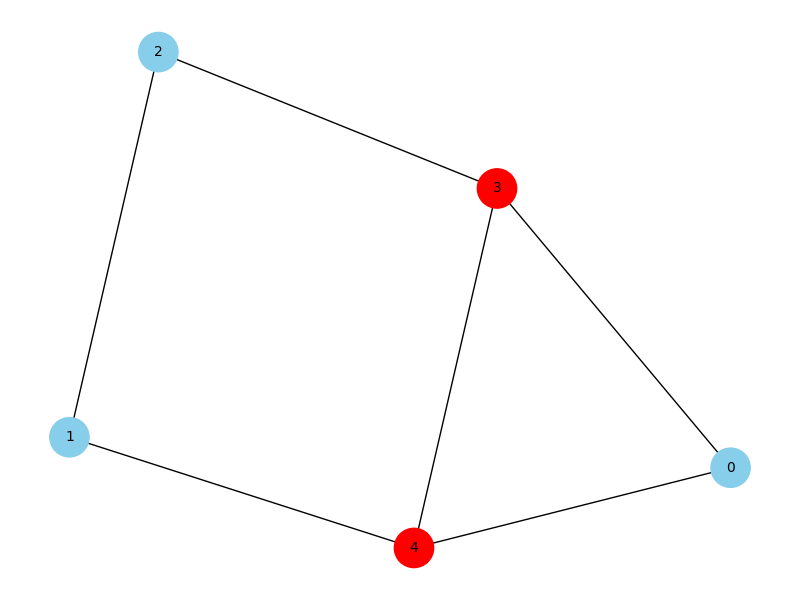
\includegraphics[width=\linewidth]{dokumentace/pic/graf_1_34.png}
                \caption{Podgraf s uzly 3 a 4.}
            \end{subfigure}
            \begin{subfigure}[b]{0.3\textwidth}
                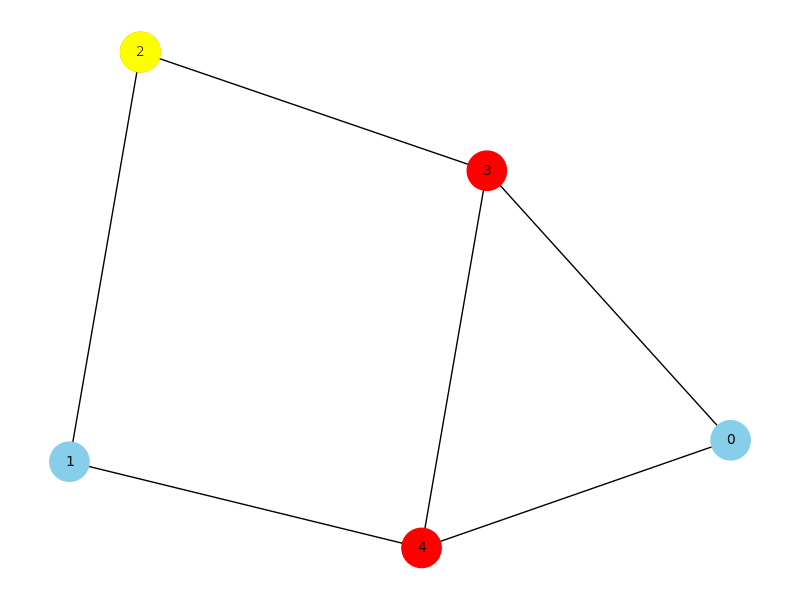
\includegraphics[width=\linewidth]{dokumentace/pic/graf_1_234_2.png}
                \caption{Přidání uzlu 2 nezachová vlastnost kliky podgrafu.}
            \end{subfigure}
            \begin{subfigure}[b]{0.3\textwidth}
                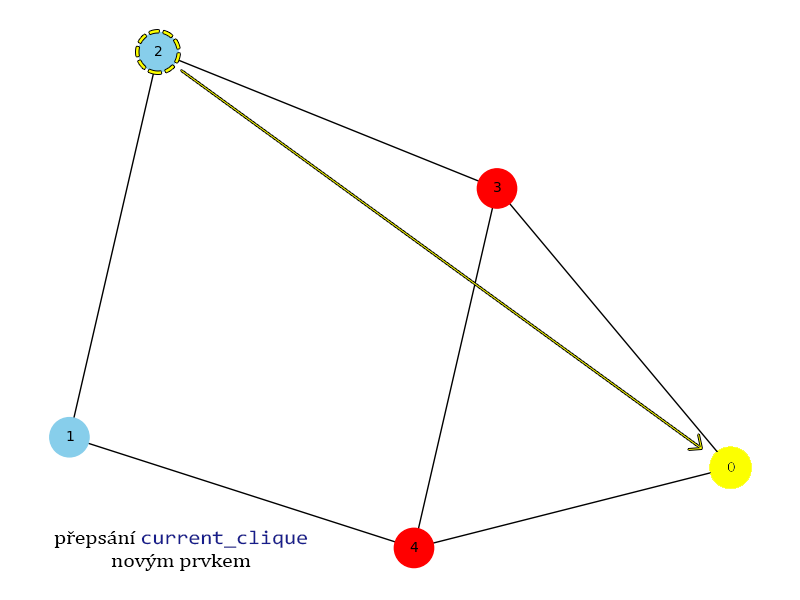
\includegraphics[width=\linewidth]{dokumentace/pic/graf_1_340.png}
                \caption{Přepis falešného uzlu kliky dalším podezřelým.}
            \end{subfigure}
            \caption{Ilustrace k přepisu uzlů v proměnné \lstinline{current_clique} pro hledání zpětným vyhledáváním (pořádí uzlů nemusí odpovídat pořadí v programu).}
            \label{fig:backtrack_imp}
        \end{figure}


\section{Experiment} \label{sec:experiment}
    Tato kapitola se zabývá experimentálním ověřením vlastností implementace algoritmů v jazyce C (kapitola \ref{sec:implem}) pro jejich následné porovnání s teoretickými předpoklady vznesenými v kapitole \ref{subsec:complexities_teo}.\\

    \noindent
    Pro tyto účely byl sepsán kód souboru \lstinline{experiment.c}. Bližší popis tohoto kódu je shrnut v komentářích souboru. Pro účely této kapitoly je důležitá funkce \lstinline{time_comparison_experiment}. Její zjednodušený kód je uveden v úryvku \ref{code:experiment}. Z tohoto úryvku vyplývá, že může být volán experiment pro různě husté grafy se zvolenými velikostmi pro oba, či jen jeden z algoritmů.\\

    \begin{lstlisting}[caption={Zjednodušený kód hlavní funkce souboru \lstinline{experiment.c} nasteven pro generaci grafů velikosti 5 až 30 s hustotou 0,5 pro algoritmus metody hrubé síly.}, captionpos=b, label={code:experiment}]
void time_comparison_experiment() {
    FILE* file = fopen("experiment.csv", "w");
    fprintf(file, "size,density,bruteforce,backtracking\n");
    for (int size = 5; size <= 30; size += 1) { 
        for (double density = 0.5; density <= 0.5; density += 0.3) {
            graph* g = generate_random_graph(size, density);

            // bruteforce
            double bruteforce_time = measure_execution_time(bruteforce, g);

            // backtracking
            // double backtracking_time = measure_execution_time(backtracking, g);

            // fprintf(file, "%d,%.2f,%.6f,%.6f\n", size, density, bruteforce_time, backtracking_time);  // pro oba algoritmy
            fprintf(file, "%d,%.2f,%.6f,na\n", size, density, bruteforce_time);  // pouze bruteforce
            // fprintf(file, "%d,%.2f,na,%.6f\n", size, density, backtracking_time);  // pouze backtracking

            graph_delete(g);
        }
    }
    fclose(file);
}
    \end{lstlisting}

    \noindent
    Důležitou poznámkou je, že funkce \lstinline{measure_execution_time}, která měří délku časového intervalu potřebného pro nalezení všech řešení, používá standardní knihovnu \lstinline{time.h} a v ní funkci \lstinline{clock}. Přesnost této metody závisí na čase využitém procesorem, předpokládáme rozlišení metody větší než $\mu$s. Proto právě $\mu$s byly stanoveny jako rozlišení experimentů.\\

    \noindent
    Kód souboru \lstinline{experiment.c} byl spouštěn pro následující podmínky a algoritmy, kde $n$ vyjadřuje počet uzlů, $\rho$ hustotu hran v matici (viz kapitolu \ref{subsec:graph_imp}):
    \begin{enumerate}
        \item $\forall n \in \left<30;300\right> \cap \mathbb{N}$, $\rho = 0,5$, algoritmus metody zpětného vyhledávání
        \item $\forall n \in \left<5;30\right> \cap \mathbb{N}$, $\rho = 0,5$, algoritmus metody hrubé síly
        \item $\forall n \in \left<5;59\right> \cap \mathbb{N}$, $\forall \rho \in \bigcup_{k=1}^{9}0,1\cdot k$, algoritmus metody zpětného vyhledávání
        \item $\forall n \in \left<5;92\right> \cap \mathbb{N}$, $\forall \rho \in \bigcup_{k=1}^{9}0,1\cdot k$, algoritmus metody hrubé síly
    \end{enumerate}

    \subsection{Srovnání závislosti časové náročnosti algoritmů na počtu uzlů $n$}
        Tato podkapitola se zabývá výsledky z experimentů výše označených jako 1. a 2. Díky vhodnému nastavení kódu souboru \lstinline{experiment.c} byla získána data délek časových intervalů potřebných k nalezení řešení úlohy hledání největší kliky v závislosti na počtu uzlů $n$ vstupního neorientovaného grafu. Závislosti pro oba tyto algoritmy jsou vyneseny na obrázku \ref{fig:exp_n_linlin}. Protože závislost projevuje exponenciální charakter a výstup mění řád mnohem rychleji než vstup, byla tato data vynesena i v logaritmickém měřítku, to je zachyceno na obrázku \ref{fig:exp_n_loglog}.

    \subsection{Srovnání závislosti časové náročnosti algoritmů na počtu uzlů $n$ a hustotě matice sousednosti}
        Tato podkapitola se zabývá výsledky z experimentů výše označených jako 3. a 4. Na základě těchto experimentů byly vykresleny dvě teplotní mapy srovnávající vliv počtu uzlů $n$ a hustoty matice sousednosti na časový interval potřebný k nalezení všech řešení. Protože výsledná data vykazují exponenciální chování, byl vynesen tentýž graf také v logaritmickém měřítku. Na něm byly nulové body zanedbány. Zmíněné grafy jsou na obrázcích \ref{fig:n_rho_lin} a \ref{fig:n_rho_log}.

    \subsection{Vyhodnocení experimentu}
        Experimenty srovnávající délku časového intervalu pro vyřešení úlohy v závislosti na velikosti matice sousednosti $n$ mezi algoritmy, jež byly provedeny s hustotou této matice o hodnotě $\frac{1}{2}$, prokázaly předpokládané chování (podle teoretických předpokladů z kapitoly \ref{subsec:complexities_teo}), a to sice, že algoritmus metody hrubé síly je z dvou porovnávaných více časově náročný.\\
        
        \noindent
        Je patrné, že se oba algoritmy chovají exponenciálně, což vychází z vlastností implementace matice sousednosti (kapitola \ref{subsec:graph_imp}). Rozdíl je však v horní hranici časových složitostí. V kapitole \ref{subsec:complexities_teo} byl vznesen předpoklad, že metoda hrubé síly má tuto funkci $n$-krát větší než metoda zpětného vyhledávání. I experiment potvrzuje tuto vlastnost.\\

        \noindent
        Další metoda, kterou by bylo možné přesněji ověřit shodu s předpokladem časové složitosti, by bylo vyjádřit limitu poměru logaritmizovaných časových intervalů. To vyplývá z následujících rovnic:

        \begin{equation}
            \begin{aligned}
                \text{Pro hrubou sílu: }&\log{\left(n^2\cdot 2^n\right)} = 2\log{\left(n\right)}+n\log{\left(2 \right)} = f(n)\\
                \text{Pro zpětné vyhledávání: }&\log{\left(n\cdot 2^n\right)} = \log{\left(n\right)}+n\log{\left(2 \right)} = g(n)
            \end{aligned}
        \end{equation}

        \noindent
        Protože se výrazy liší pouze o koeficient 2 u jednoho ze sčítanců, jakýsi pomyslný vliv tohoto koeficientu bude s $n \rightarrow \infty$ klesat, a tak bude čitatel i jmenovatel nabývat téže hodnoty. Tento jev je shrnut v rovnici \ref{eq:frac_lim} a obrázku \ref{fig:log_frac}.
        
        \begin{equation} \label{eq:frac_lim}
            \lim_{n\to\infty}\frac{f(n)}{g(n)} = 1
        \end{equation}

        \noindent
        Toto srovnání však v rámci experimentu neproběhlo, jelikož vybraná implementace (viz kapitolu \ref{sec:implem}) má kvůli vysoké prostorové složitosti (viz kapitolu \ref{subsec:complexities_teo}) problémy s velkými maticemi a pro hustotu matice 0,5 je tedy problematické najít takovou velikost této matice, pro níž by nedetekovatelně rychlý algoritmus zpětného vyhledávání byl vykonán v měřitelném čase spolu s paměťově náročným algoritmem hrubé síly.

        \noindent
        V rámci experimentů 3. a 4. bylo na základě dat na obrázcích \ref{fig:n_rho_lin} a \ref{fig:n_rho_log} zjištěno, pro jaké neorientované grafy jsou navržené algoritmy vhodné. Protože graf pro algoritmus metody hrubé síly vykazuje relativně oproti druhému algoritmu nezávislost na hustotě matice sousednosti, můžeme učinit závěr, že je tento algoritmus univerzálnější, zatímco algoritmus metody zpětného vyhledávání je efektivní, pokud není matice zaplněna s hustotou $< 0,7$. Pro hustotu 0,9 dokonce velmi silně zaostává za algoritmem hrubé síly.
    

        \newpage
        \begin{figure}[H]
            \centering
            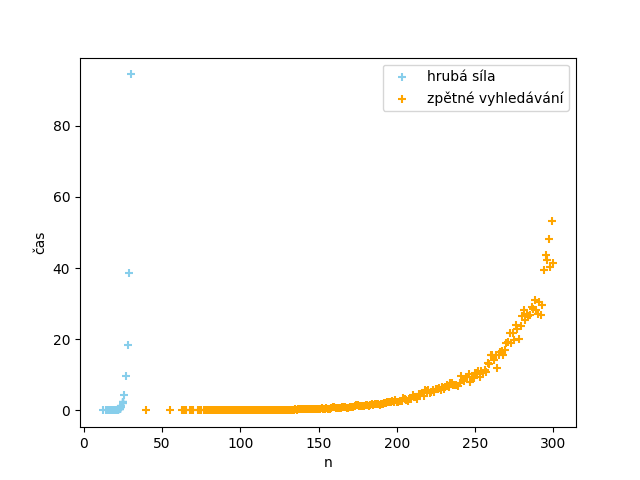
\includegraphics[width=.8\linewidth]{dokumentace/exp_vyhodnoceni/exp_lin_lin.png}
            \caption{Výsledek experimentálního měření závislosti délky časového intervalu pro dokončení úlohy na počtu uzlů vstupního grafu pro oba algoritmy.}
            \label{fig:exp_n_linlin}
        \end{figure}

        \begin{figure}[H]
            \centering
            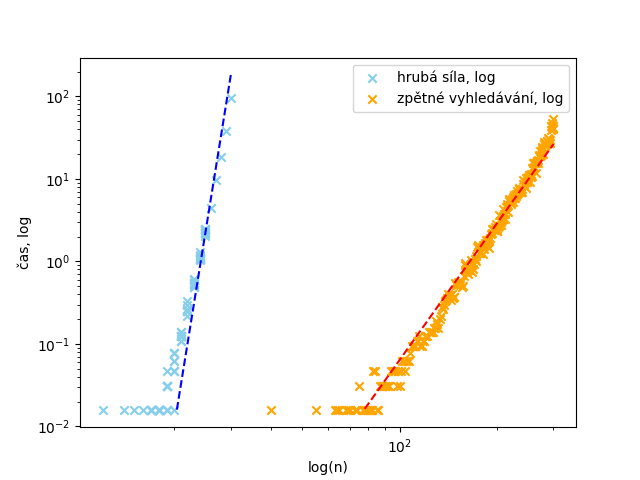
\includegraphics[width=.8\linewidth]{dokumentace/exp_vyhodnoceni/exp_log_log.png}
            \caption{Výsledek experimentálního měření závislosti délky časového intervalu pro dokončení úlohy na počtu uzlů vstupního grafu pro oba algoritmy s logaritmickým škálováním na osách.}
            \label{fig:exp_n_loglog}
        \end{figure}
        
        \begin{sidewaysfigure}
            \centering
            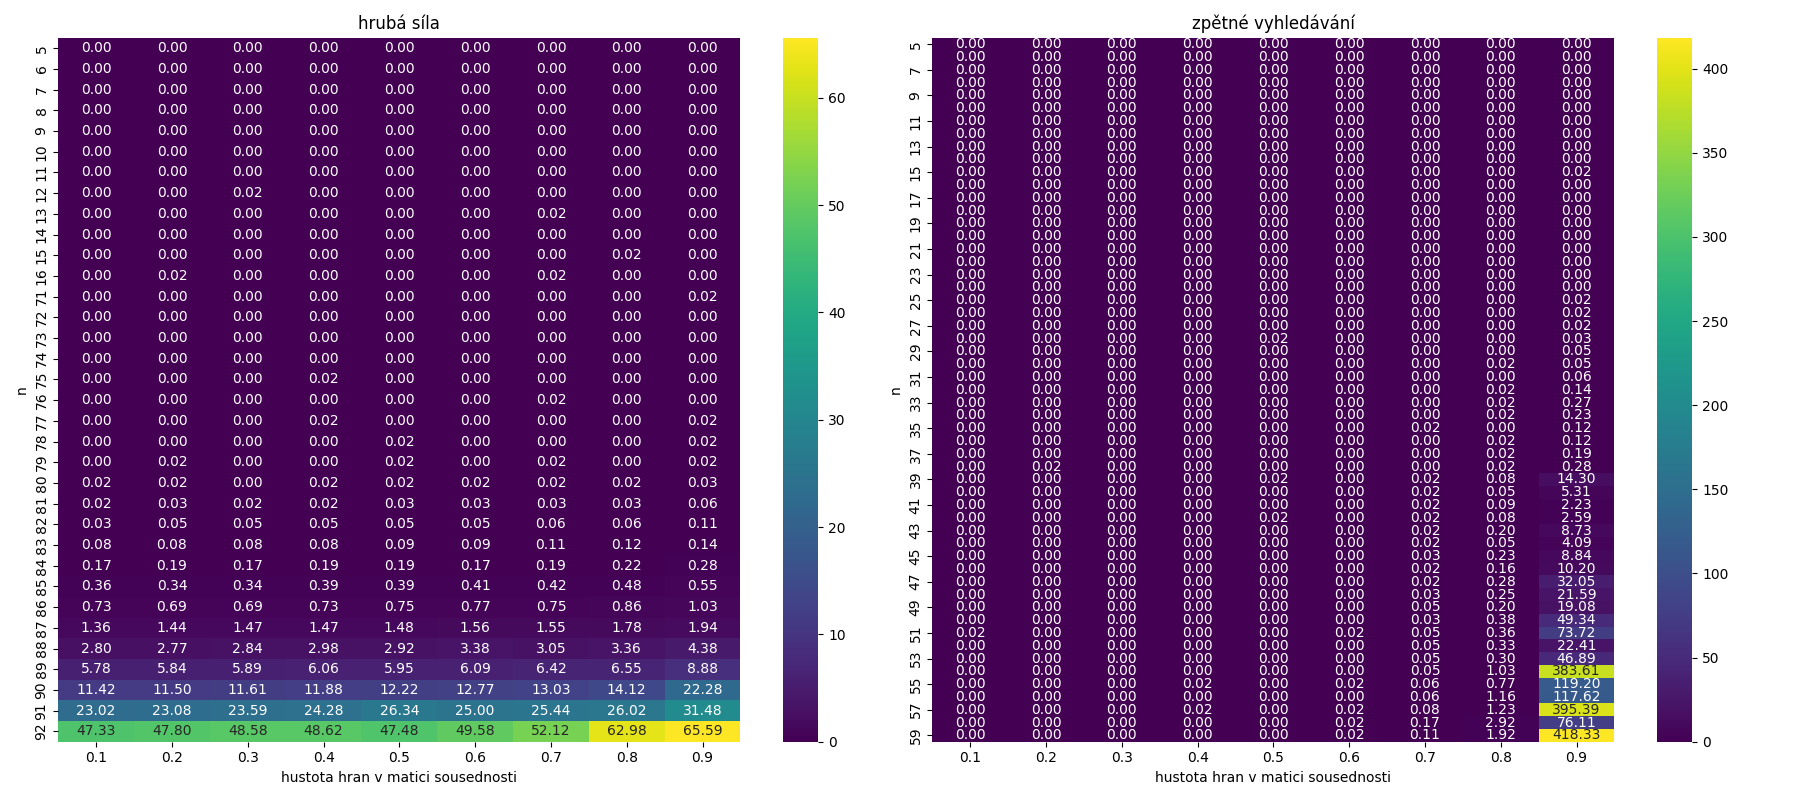
\includegraphics[width=1\textwidth]{dokumentace/exp_vyhodnoceni/n_dens.png}
            \caption{Graf závislosti časové náročnosti algoritmů na počtu uzlů $n$ a hustotě matice sousednosti.}
            \label{fig:n_rho_lin}
        \end{sidewaysfigure}

        \begin{sidewaysfigure}
            \centering
            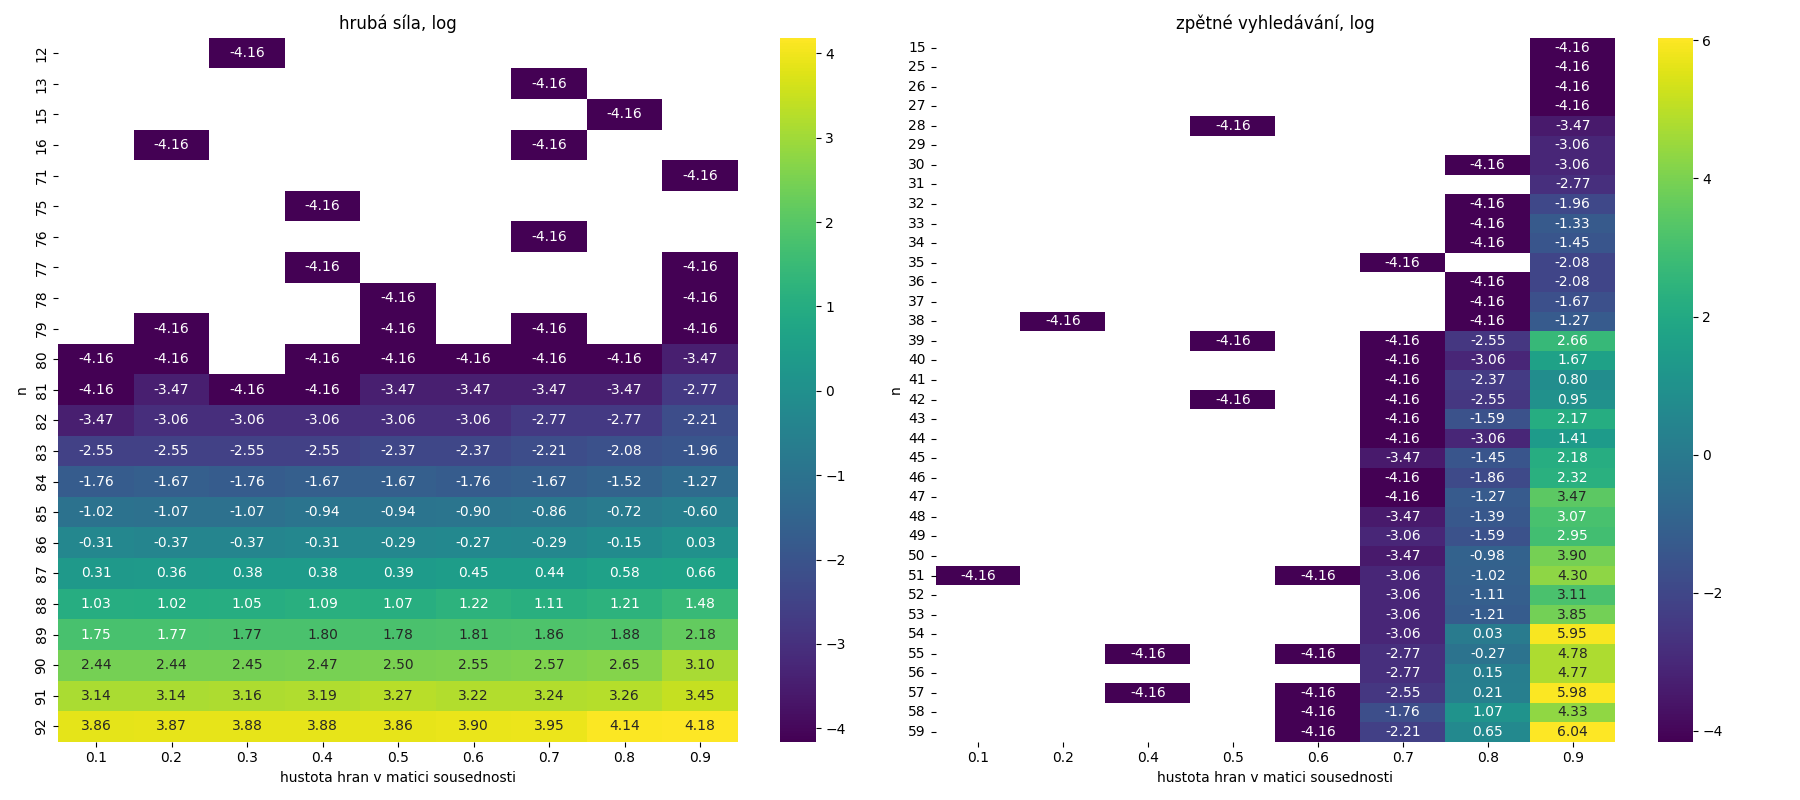
\includegraphics[width=1\textwidth]{dokumentace/exp_vyhodnoceni/log_n_dens.png}
            \caption{Graf závislosti časové náročnosti algoritmů na počtu uzlů $n$ a hustotě matice sousednosti v logaritmickém měřítku.}
            \label{fig:n_rho_log}
        \end{sidewaysfigure}

        \begin{figure}
            \centering
            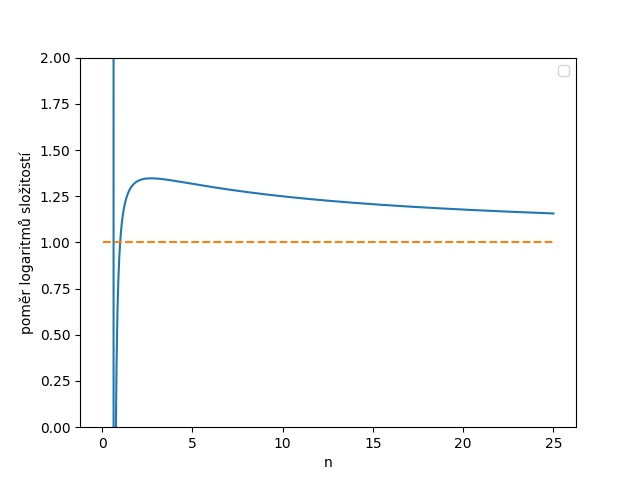
\includegraphics[width=0.8\linewidth]{dokumentace/exp_vyhodnoceni/log_frac.png}
            \caption{Závislost poměru horních hranic logaritmů složitostí obou algoritmů na velikosti matice sousednosti $n$.}
            \label{fig:log_frac}
        \end{figure}

\section{Závěr}
    Byl vytvořen jednoduchý program v jazyce C, který implementuje dva způsoby hledání všech největších klik v neorientovaném grafu. Těmito způsoby jsou použití metody hrubé síly a metody zpětného vyhledávání. Implementace těchto metod je shrnuta v kapitole \ref{sec:implem}. V téže kapitole je implementace neorientovaných grafů maticí sousednosti.\\

    \noindent
    Pro oba vybrané algoritmy byly stanoveny časové a prostorové složitosti teoreticky v kapitole \ref{subsec:complexities_teo}. Teoretické výroky byly nakonec experimentálně ověřeny pomocí programu v jazyce C. Postup i výsledky tohoto měření jsou uvedeny v kapitole \ref{sec:experiment}. V jejich dvou sekcích jsou pak stanoveny závěry rozebírající časovou náročnost a vhodnou aplikaci každé metody.\\

    \noindent
    Kapitola \ref{sec:experiment} pak také nastiňuje možnosti další optimalizace či metody přesnější analýzy zkoumaných dat, které nejsou obsahem této práce.
    

    
\bibliographystyle{plain}
\bibliography{dokumentace/zdroje/lib}
\newpage
\lstlistoflistings
\listoffigures
\end{document}